\documentclass[12pt]{article}
\setcounter{secnumdepth}{0}
\usepackage{amsmath}
\usepackage{txfonts}
\usepackage{setspace}
\usepackage{xcolor}
\usepackage{titlesec}
\usepackage[left=1in, right=0.59in, top=0.79in, bottom=0.79in]{geometry}
\usepackage{graphicx}
\usepackage{float}
\usepackage[utf8x]{inputenc}
\usepackage{hyperref}

\setstretch{1.15}
\definecolor{sectioncolor}{RGB}{0,102,204}
\definecolor{subseccolor}{RGB}{0,102,204}


\titleformat{\section}[block]{\color{sectioncolor}\bfseries\large}{}{0pt}{}


\begin{document}











	\begin{figure}[h!]
		\centering
		
\includegraphics[width=1\textwidth]{assets/images/header.png}
		
	 \end{figure}

     \begin{figure}[H]
        \raggedleft
        
\includegraphics[width=0.5\textwidth]{assets/images/banm.png}
        % \caption{Right-aligned Image}
        % \label{fig:right_aligned_image}
      \end{figure}

      \begin{center}
        {\fontsize{20pt}{20pt}\selectfont 

        \vspace{10mm}
            Baku Higher Oil School

            Chemical Engineering Department

            Process Engineering A

            EACOP Project
        }
      \end{center}
      \begin{center}
        {\fontsize{14pt}{14pt}
        \raggedright
        \vspace{30mm}
            Team name: Crude Crusaders \\

            Team members: Ruhan Farajov, Sultanmurad Safarov, Farid Bayramov, Seymur Safarov \\

            Project title: East African Crude Pipeline \\

            Date of Submission: 21.11.2023 \\

            Supervisor: Rashad Nazaraliyev \\

            
        }
      \end{center}




     \newpage
     \tableofcontents
     \newpage
	

      \section{Abstract}

      {\fontsize{12pt}{12pt}

      \hspace*{1em} The project is objected to provide a solution to the transportation of crude oil in the East Africa, addressing the need of the energy sources throughout the region as well as crude oil export to other countries. The study considers the most important topics to take into account in the implementation of the project, such as route, pipe, and pump design. The results reveal the turbulent flow regime, a higher available NPSH value compared to the required one, indicating that the calculations are made correctly. The report is a valuable resource to comprehend technical and operational aspects of the project.
      }

      \section{Introduction}

      {\fontsize{12pt}{12pt}

      \hspace*{1em} The most predominant culprit behind the implementation of the East African Crude Oil Pipeline (EACOP) project is solving the problems pertained to the transportation of in the East African region, such as logistical challenges, environmental risks and increased costs$^{[1]}$. This project study aims to demonstrate ways forward to the above-mentioned problems by shedding some light on the background work in implementing the project which meets the energy demand of the region in a sustainable way. 

      The most essential focus of the study is the methodology utilized in the design and realization of the EACOP project. Notably, useful geospatial analysis tools like Google Earth Pro are used to select the best route, ensuring the efficiency of the pipeline and alleviating environmental harm. Moreover, the pipe and pump designs are considered carefully, maintaining the industry standards and adding safety aspects for better performance. The most crucial advantages in using this methodology is operational efficiency, lessened impact on the environment, ad ensured economic viability.

      Throughout the document, the subsequent sections will highlight the detailed information about the project:

      1. \textbf{Problem Statement} : the identification of the problem in the field and the reasons for the implementation.

      2. \textbf{Methodology}: a detailed explanation of the theory behind the calculations.

      3. \textbf{Results and Applications}: A comprehensive demonstration of the acquired calculations.

      4. \textbf{Discussion}: a meticulous analysis of the obtained results, and recommendations for future development.

      5. \textbf{Conclusion}: the summation of all the essential findings and the overall importance of the project in tackling the regional energy transition problems. 
      }


      \section{Problem statement}
      {\fontsize{12pt}{12pt}

      \hspace*{1em} The East African Crude Oil Pipeline (EACOP) is aimed to tackle the urgent demand for a reliable infrastructure to transport crude oil throughout the region. The lack of a particular pipeline system has caused logistical challenges, environmental problems, and higher transportation costs as a consequence of the other means of oil transfer$^{[2]}$. Additionally, the absence of the dedicated energy sources in most parts of the region has increased the demand for a sustainable solution. \\

      To address these problems, a comprehensive approach has been used, implementing useful tools such as Google Earth Pro for the route design as well as taking the sustainability problems into account. Using the pump and pipe sizing methodologies, the most essential details of the pipeline such as pump configurations and pipe specifications have been carefully ascertained and validated utilizing a standard engineering software called Aspen HYSYS. \\

      }


      \section{Methodology}
      {\fontsize{12pt}{12pt}

      \hspace*{1em} In the following section of the report, the main theory behind all the calculations made will be introduced together with the equations utilized. The aim of paramount importance in giving this project to engineering students is to enhance their technical and soft skills and research habits. \\
      \hspace*{1em} The project aims to transfer Uganda oil to Tanzania through which the oil could be transported to Europe and other parts of the world. To implement the project, there are 5 important topics to consider. They are highlighted as follows: \\
      \hspace*{1em}1.	Pipe sizing – choosing the right material for the pipe, its parameters, and effectiveness. \\
      \hspace*{1em}2.	Pump design – selecting the most appropriate pump based on the calculations. \\
      \hspace*{1em}3.	Route design – figuring out the most suitable way to construct the pipeline . \\
      \hspace*{1em}4.	Economic side – computing the cost of the project, and increasing the revenue. \\
      \hspace*{1em}5.	Environmental sustainability – taking this into account is crucial to lessen the environmental impact related to the extraction, production, and transportation of fossil fuels. \\

      }
      \subsection{Route design: }
      {\fontsize{12pt}{12pt}

      The route design should be done by taking various factors into account: \\
      \hspace*{1em}1.	Geographical terrain – it is necessary to asses the changes in the elevation to minimize the cost, and additionally, the soil composition should also be considered to make sure the strong fundamentals for the pipeline. \\
      \hspace*{1em}2.	Environmental impact – the environmentally sensitive areas like wildlife habitats and protected areas should not be crossed, and the water crossing should be avoided as much as feasible to protect the aquatic life and water quality. \\
      \hspace*{1em}3.	Human settlements – it is crucial to evade passing the pipeline from the densely populated areas, and from the cultural or historical places. \\
      \hspace*{1em}4. Safety and Security – the areas with a high probability to experience natural disasters should be avoided, and also, the security concerns need to be assessed to protect the pipeline from any threads.  \\

      }
      \subsection{Pipe design: }
      {\fontsize{12pt}{12pt}

      \hspace*{1em} Taking into account that the oil of Uganda is waxy and the pipeline system will operate under a relatively high temperature (50oC) and pressure (20 psi), its material is chosen to be carbon steel for the reasons outlined below: \\
      \hspace*{1em}• 	Strength and Resistance – These types of pipes demonstrate high resilience and strength, leading them to resist accidents such as fair, high pressure, and high temperatures. Moreover, they are also resistance to corrosion. \\
      \hspace*{1em}• 	Cost-effectiveness – this material usually has a lower cost in comparison with the other ones, making it a preference for transportation of waxy oils, particularly in large-scale industrial projects. Furthermore, compared to its alternatives, the maintenance cost is much lower, making way for a longer lifetime of the pipelines. \\
      \hspace*{1em}• 	Availability and Standardization – a plethora of carbon steel pipe types in distinctive and standardized sizes are greatly available so that replacing them in case of a problem is extremely easy. \\
      \hspace*{1em}As the material has been chosen, it is necessary to calculate the optimum diameter based on the equation illustrated below:
      \begin{center}
        % $d_{\text{optimum}} = m^0.53 * μ^0.03 * ρ^-0.37$
        $d_{\text {optimum }}=m^{0.53} \times \mu^{0.03} \times \rho^{-0.37}$ (1)


        
      \end{center}

      Where, \\
      \hspace*{1em}$d$ → optimum diameter of the pipe \\
      \hspace*{1em}$m$ → mass flow rate \\
      \hspace*{1em}$\mu$ → dynamic viscosity \\
      \hspace*{1em}$\rho$ → density of the oil \\

      As the temperature is high throughout the pipeline, expansion will take place and in order to evade this problem, the pipe inside diameter will be taken 5 \% more than the optimum diameter, and the outside diameter will be found based on this value.
      }
      \subsection{Pump design: }
      {\fontsize{12pt}{12pt}

      \hspace*{1em} Without being dependent on the type of the pump utilized, the subsequent steps ought to be fulfilled$^{[3]}$: \\
      \hspace*{1em } •	Compute the required pump head at the given flow rate. \\
      \hspace*{1em} •	Compute the available NPSH and make sure that it is more than required NPSH. \\
      \hspace*{1em} •	Resolve on any specific issues, the viscosity and corrosivity of the fluid. \\
      \hspace*{1em} •	Resolve on the prime mover, power requirement and the pump needed for the operation. \\

Any pumping station could be divided into two parts, one of which is the “suction side” including all the parts before the inlet of pump, and the “discharge side” compromising all sections after the pump. Hydrostatic and static heads help the fluid to flow into the pump, whereas frictional head losses preclude the fluid flow. The same occurs at the discharge side as well – as indicated in Figure 1.\\
In order to calculate the pump head, it is required to figure out the subtraction of section and discharge head at the given flowrate. \\




\begin{figure}[H]
  \centering
  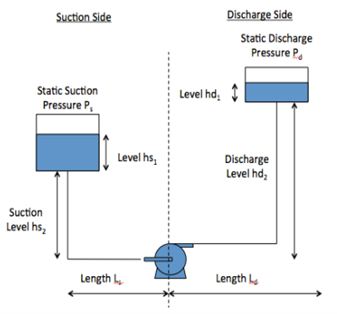
\includegraphics[width=0.5\textwidth]{assets/images/p_sys.png}
  \textit{Figure 1}
  
 \end{figure}

 The parameters of the suction side will be calculated as highlighted below: \\

Static pressure(suciton vessel): $\frac{P_s}{\rho g} (2)$ \\

Liquid level(suction vessel): $h_{s 1} (3)$ \\

Liquid level (suction vessel-pump): $h_{s 2} (4)$ \\

Straight length of pipe: $L_{s t}=h_{s 2}+L_s (5)$ \\

Equivalent length (fittings):   $L_{s e}=\sum L_e (6)$  \\

Frictional head loss (suction):  $h_{f s}=f^{\prime}\left(\frac{L_{s t}}{d}+\frac{L_{d e}}{d}\right)\left(\frac{\rho u^2}{2}\right) (7)$   \\

Total suction head:   $h_s=\frac{P_s}{\rho g}+h_{s 1}+h_{s 2}-h_{f s} (8)$  \\

The figures for the discharge should be calculated as shown followingly: \\

Static pressure (discharge vessel): $\frac{P_d}{\rho g} (9)$\\

Liquid level (discharge vessel): $h_{d 1} (10)$ \\

Liquid level (discharge vessel-pump): $h_{d 2} (11)$ \\

Straight length of pipe: $L_{s t}=h_{s 2}+L_s (12)$ \\

Equivalent length (fittings): $L_{d e}=\sum L_e (13)$ \\

Frictional head loss (discharge): $h_{f d}=f^{\prime}\left(\frac{L_{s t}}{d}+\frac{L_{d e}}{d}\right)\left(\frac{\rho u^2}{2}\right) (14)$  \\

Total discharge head: $h_s=\frac{P_d}{\rho g}+h_{d 1}+h_{d 2}-h_{f d} (8)$


Based on the analysis indicated above, the most important equations are the total heads for discharge and suction: 
\begin{center}
$h_s=\frac{P_s}{\rho g}+h_{s 1}+h_{s 2}-h_{f s}(\text { suction }) (14)$  \\

\vspace{2mm}
$h_d=\frac{P_d}{\rho g}+h_{d 1}+h_{d 2}-h_{f d}(\text { discharge }) (15)$ \\

\end{center}

After determining these two parameters, the pump head could be ascertained by subtracting suction from the discharge head: 
\begin{center}
$\Delta h_p=h_d-h_s(16)$ \\
\end{center}

In order to avoid cavitation, it is crucial to calculate Net Positive Suction Head, and ensure that it is more than required head (8m in this case): 
\begin{center}
Available NPSH $=\frac{P_s-P^{s a t}}{\rho g}+h_{s 1}+h_{s 2}-h_{f s} (17)$ \\

\end{center}

The minimum power required to drive fluid through the pump is the multiplication of the flowrate and the pump pressure drop which is ascertained with the help of pump head: \\

Nevertheless, the input of the power for driving the pump is dependent on the pump efficiency $\eta$: \\

\begin{center}

$\dot{W}_{\imath n}=\frac{\rho g \Delta h_p Q}{\eta} (19)$
\end{center}

      }
      \section{Results and applications}
      {\fontsize{12pt}{12pt}
      \hspace*{1em} In this section of the report, the results acquired from the calculations based on the equations mentioned in the methodology section will be outlined together with tables. 

      Table 1 illustrates the data about the parameters required to conduct the pump and pipe design:
      }

      
\begin{table}[H]
  \centering
  \begin{tabular}{|l|c|c|c|}
    \hline
    \multicolumn{4}{|c|}{Quantities for the route and crude oil} \\
    \hline
    \textbf{Parameters} & \textbf{Symbols} & \textbf{Values} & \textbf{Units} \\
    \hline
    \textbf{Length} & $l$ & 155.46 & $km$ \\
    \hline
    \textbf{Diameter} & $d$ & 0.592 & $m$ \\
    \hline
    \textbf{Inside diameter} & $d(inside)$ & 621.6 & $mm$ \\
    \hline
    \textbf{Outside diameter} & $d(outside)$ & 654.2 & $mm$ \\
    \hline
    \textbf{Pipe thickness} & $t$ & 16.3 & $mm$ \\
    \hline
    \textbf{Cost of 12 metres of carbon steel pipeline} & & 100 & USD \\
    \hline 
    \textbf{Cost for the whole carbon steel pipeline} & & 12.971 & million USD \\
    \hline
    \textbf{Number of pumps} & & 6 & \\
    \hline
    \textbf{Cost of one pump} & & 560 & USD \\
    \hline
    \textbf{Temperature} & $T$ & 51 & $^\circ$C \\
    \hline
    \textbf{Saturation pressure} & $P_{sat}$ & 210 & $kPa$ \\
    \hline
    \textbf{Approximate cost of construcion} & & 12.974 & million USD \\
    \hline
    \textbf{Density} & ${\rho}$ & 870 & $kg/m^3$ \\
    \hline
    \textbf{Dynamic viscosity (at 50 $^\circ$)} & $\mu$  & 0.02094 & $Pa*s$ \\
    \hline
    \textbf{Kinematic viscosity (at 50 $^\circ$)} & $\nu$ & 24.069 * $10^{-6}$   & $m^2/s$ \\
    \hline
    \textbf{Capacity of pipeline} & $Q$ & 216000 & $barrels/day$ \\
    \hline
    \textbf{1 barrel} & & 0.16 & $m^3$ \\
    \hline
    \textbf{Volumetric flow rate} & $Q$ & 0.4 & $m^3/s$ \\
    \hline
    \textbf{Mass flow}  & $m$ & 348 & $kg/s$ \\
    \hline
    \textbf{Flow speed} & $\nu$ & 1.453 & $m/s$ \\
    \hline
    \textbf{Reynolds number} & $Re$ & 35743.00 & - \\
    \hline
    \textbf{Moody friction factor} & $f'$ & 0.0410 & - \\
    \hline
    \textbf{Absolute roughness for steel pipe} & $\varepsilon$ & 0.0675 & $m$ \\
    \hline
    \textbf{Relative roughness} & $k$ & 0. 114 & - \\
    \hline
    \textbf{Frictional pressure drop along whole pipeline} & $\Delta{P_{fr}}$ & 198.0 & $MPa$ \\
    \hline
    \textbf{Elevation at starting point (Hoima)} & $h_{initial}$ & 1119 & $m$ \\
    \hline
    \textbf{Elevation at ending point (Tanga Port)} & $h_{final}$ & 20 & $m$ \\
    \hline
    \textbf{Pressure gradient} & PG & 121.2170007 & $Pa/m$ \\
    \hline
    \textbf{Total pressure drop (resulting from elevations and friction)} & $\Delta{P_{total}}$ & 188.67 & $MPa$ \\
    \hline
    \textbf{Acceleration due to gravity} & $g$ & 9.81 & $m/s^2$ \\
    \hline

  \end{tabular}
  \raggedright
  \vspace{2mm}

  \textit{Table 1: quantities for the route and the crude oil}
  \label{tab:table_with_line_breaks}
\end{table}

{\fontsize{12pt}{12pt}

\hspace*{1em} As it can be seen from the table, the optimum diameter is calculated to be 592 mm, while the inside diameter of the pipe is chosen to be 621 mm, which is 5 \% more than the latter to avoid the expansion of the pipe in higher operating conditions. As for the Reynolds number, it is found to be 35743, indicating the turbulent flow regime. \\

Table 2 highlights the information about the first pumping station system: \\
}
\begin{table}[H]
  \centering
  \begin{tabular}{|c|c|c|c|}
    \hline
    \multicolumn{4}{|c|}{\textbf{Suction head}} \\
  
    \hline
     \textbf{Parameters} & \textbf{Symbols} & \textbf{Values} & \textbf{Units}\\
    \hline
    \textbf{Suction pressure} & $P_{s}$ & 137895 & $Pa$ 
    \\
    \hline
    \textbf{Elevation from pump} & $h_{el}$ & 20 & $m$ \\
    \hline

    \textbf{Minor loss head} & $h_{minor}$ & 0.21527 & $m$ \\
    \hline
    \textbf{Major loss head} & $h_{majoe}$ & 0.223634 & $m$ \\
    \hline
    \textbf{Pressure loss head} & $h_{fs}$ & 0.438904 & $m$ \\
    \hline
    \textbf{Head due to suction pressure} & $h_{sp}$ & 16,15698 & $m$ \\
    \hline
    \textbf{Sum of K values} & $\sum{K}$ & 2 & - \\
    \hline
    \textbf{Length} & $L$ & 30 & $m$ \\
    \hline
    \textbf{Total Suction Head} & $h_{s}$ & 35.71808 & $m$ \\
    \hline
    \multicolumn{4}{|c|}{\textbf{Discharge head}} \\
    \hline
    \textbf{Discharge pressure} & $P_d$ & 150000 & $Pa$ \\
    \hline
    \textbf{Elevation from pump} & $h_{el}$ & 66 & $m$ \\
    \hline
    \textbf{Minor loss head} & $h_{minor}$ & 0.285233 & $m$ \\
    \hline
    \textbf{Major loss head} & $h_{major}$ & 2622.272& $m$ \\
    \hline
    \textbf{Pressure loss head} & $h_{fd}$ & 2622.558 & $m$ \\
    \hline
    \textbf{Head due to discharge pressure} & $h_{dp}$ & 17,57531 & $m$ \\
    \hline
    \textbf{Sum of K values} & $\sum{K}$ & 2.65 & - \\
    \hline
    \textbf{Length} & $L$ & 351772 & $m$ \\
    \hline
    \textbf{Total discharge head} & $h_d$ & 2706.133 & $m$ \\
    \hline
    \multicolumn{4}{|c|}\textbf{Pump characteristics} \\
    \hline
    \textbf{Pump head} & $h_p$ & 2670.415 & $m$ \\
    \hline
    \textbf{Pressure drop} & $\Delta$P & 22791190 & $Pa$ \\
    \hline
    \textbf{Outlet pressure of pump} & $P_p$ & 22941190 & $Pa$ \\
    \hline
    \textbf{Effective power} & $W$ & 9116476 & $W$ \\
    \hline
    \textbf{Efficiency} & $\eta$ & 90 & $\%$ \\
    \hline
    \textbf{Motor power} & $W_m$ & 10129418 & $W$ \\
    \hline
    \textbf{Total suction head} & $h_s$ & 35.71808 & $m$ \\
    \hline
    \textbf{Total discharge head} & $h_d$ & 2706.133 & $m$ \\
    \hline
    \textbf{NPSH(required)} & $H_{req}$ & 8 & $m$ \\
    \hline
    \textbf{NPSH(available)} & $H_{ava}$ & 11.11264 & $m$ \\
    \hline
  \end{tabular}
  
  \label{tab:vertically_merged_cells_table}
\end{table}
\vspace{2mm}
\textit{Table 2}
\vspace{3mm}

{\fontsize{12pt}{12pt}

\hspace*{1em} What stands out from the table is that the figure for pump head is approximately 2670 m, and as it is so high, one pump is not enough to drive this fluid. Due to that a pump station with the power close to 10 MW is required to be established. Coming to the NSPH values, the available one is more than the required figure, at 11.11 m and 8 m respectively, indicating that cavitation will not take place. 

Another important point to annotate is that, after the pump stations, the elevation of the pipeline system decreases in a sharp trend, thus the pressure increases considerably. To overcome this problem, 2 pressure reduction stations should be installed. With the help of the engineering software, Aspen HYSYS, the pipeline system together with the pump and pressure reduction stations has been drawn: \\

\begin{figure}[H]
  \centering
  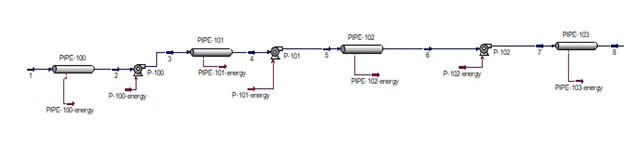
\includegraphics[width=1\textwidth]{assets/images/design1.jpg}
  \textit{Figure 2: the first 3 pump stations of the pipeline}
  
 \end{figure}

 \begin{figure}[H]
  \centering
  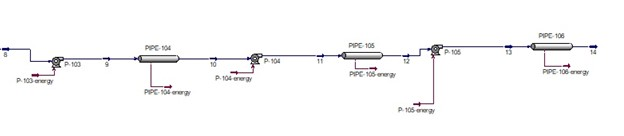
\includegraphics[width=1\textwidth]{assets/images/design2.jpg}
  \textit{Figure 3: the rest of the pipeline}
  
 \end{figure}
 {\fontsize{12pt}{12pt}

 The route has been drawn by taking all the important details mentioned in the methodology section of the report. The designated route is illustrated as follows: \\
 }

 \begin{figure}[H]
  \centering
  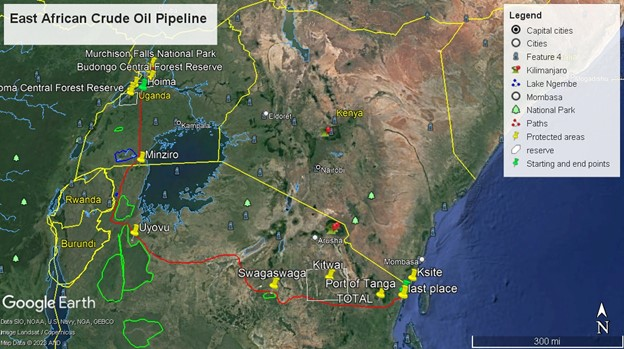
\includegraphics[width=1\textwidth]{assets/images/route.jpg}
  \textit{Figure 3: the route of the pipeline}
  
 \end{figure}
}
      \section{Discussion}

      \hspace*{1em}In this part of the report, the data presented in the preliminary section will be thoroughly analysed. The garnered results from the pump and pipe design for the project are relatively appropriate to implement the project. As for the table 1, it is apparent that the total length of the pipeline system is drawn to be 1556 km connecting the Hoima to Tanga port. Although the optimum diameter is calculated as 592 mm, the selected pipe is 621 mm (5\% more) to mitigate the potential expansion problems under higher temperature and pressures. The total pressure drop is around 188.67 MPa, while the Reynolds number with the value of 35,743 shows the turbulent flow regime, being suitable to the requirements in the oil transportation. 

      \hspace*{1em}Coming to the table 2, based on the discharge and the suction head, the pump head and the overall pressure loss are ascertained as 2760.12 m and 22MPa in turn. The power required to operate the system is 9.11 MPa; however due to the 90 \% efficiency of the pump, 10.1 MPa should be provided to the system. Another most striking point to highlight is that the NPSH available is more than the NPSH required, thus it could be denoted that the cavitation will not take place.\\
      \section{Conclusion}

      In conclusion, the careful study of the East African Crude Oil Pipeline (EACOP) project is done, examining the pipeline, pump stations, and other factors for a strong implementation. The 1556 km route is designed with attention to geography and the environment, aligning with project goals. The detailed design, including a 621 mm diameter, addresses potential thermal expansion. The Reynolds number of 35,743 ensures efficient turbulent flow for oil transport$^{[4]}$. The study reveals a delicate balance of factors affecting system efficiency, with a pump head of 2760.12 m and an overall pressure loss of 22 MPa. It is needed to consider energy use and operational costs, focusing on preventing cavitation through NPSH analysis. While questions about long-term sustainability persist, exploring energy efficiency, pump station distribution, and environmental impact offers ways to improve. Ongoing research could introduce advanced materials and technologies for a stronger and more efficient EACOP infrastructure.
      
      \section{References}
      \textbf{} 

      1. \url{https://eacop.com/}. (n.d.). \\

      2. Features/benefits of pipeline transportation – why pipelines are needed (2019). (n.d.). \url{https://ifsolutions.com/features-benefits-of-pipeline-transportation-why-pipelines-needed/}. \\

      3. University, H. W. (2016). Process Engineering A. Baku. \\

      4. Cimbala, Y. A. (n.d.). Fluid Mechanics. Fundamentals and Applications. . Page 325, 341, 579. \\

      5. Ltd, W. E. (n.d.). Engineering, Procurement, construction management, commisioning. \\

      6. Bidmus, Hamid \& Chau, James \& Dechant, Kenton. (2019). Absolute Roughness of Pipes from Different Manufacturing and Treatment Methods and Impact on Pipeline . (n.d.).


\end{document}